% Document uses 12 pt font
% 1 in margins
% Contains a relative path for images

\documentclass [10pt]{article}

% page geometry 
\usepackage[margin=1in]{geometry}
\usepackage{changepage}


% ----------  PACKAGES START ------------ %

% Table cell color package and highlighting
\usepackage[table]{xcolor}
\usepackage{color,soul}
\usepackage{colortbl}
\usepackage{float}
\usepackage{wrapfig}
\usepackage[rightcaption]{sidecap}
\usepackage{subfigure}
\usepackage{caption}
% VIC title package
\usepackage{cabin}
\usepackage[T1]{fontenc}

% default font package
%\usepackage{times}
\usepackage{helvet}
%\renewcommand{\familydefault}{\sfdefault}

% ---------- End Font Packages -------------- %

% Title Packages
\usepackage{titlesec}
\usepackage{titletoc}

% Image Package
\usepackage{graphicx}

% Table Packages
\usepackage{longtable}
\usepackage{multirow}
\usepackage{multicol}
\usepackage{multirow}
\usepackage{array}
\usepackage{tabularx}
\renewcommand{\arraystretch}{1.2}% Spread rows out evenly in table
\setlength{\LTpre}{0.5pt} % Reduces white space around tables (top)
%\setlength{\LTpost}{0pt} % Reduces white space around tables (bottom)
\setlength\arrayrulewidth{1pt}




% Color Packages
\usepackage{color}   
\definecolor{sectionC}{rgb}{0.016,0.227,.365}
\definecolor{subsectionC}{rgb}{.87,0.87,.87}
\definecolor{subsubsectionC}{rgb}{.94,.93,.90}
\definecolor{tableCell}{rgb}{.96,.95,.90}


% List package
\usepackage{enumitem}
\setenumerate{nosep=0pt, itemindent=0in,leftmargin=.1in, topsep= 2pt,  label = -}


% Paragraph parameter

\setlength{\parindent}{0pt}


% ------------- Creates a linked Table of Contents  Start --------------- %
\usepackage{hyperref}
\hypersetup{
colorlinks=true, %set true if you want colored links
linktoc=all,     %set to all if you want both sections and subsections linked
linkcolor=black,}  %choose some color if you want links to stand out

% ------------- Creates a click-able Table of Contents  End--------------- %

% ---------- PACKAGES END ------------ %



% ------------------- START HEADER AND FOOTER ---------------------------%
\usepackage{fancyhdr}

% Helps with the n of total n pages
\usepackage{lastpage}

\pagestyle{fancy}

% Header
\lhead{Verification and Validation } 
\rhead{Revision: 0}
\fancyhead[LE, CO]{VIC - Group 6}

% Removes line under the header 
\renewcommand{\headrulewidth}{0pt}
\setlength{\headsep}{.2in}

% Footer 

% Set the right side of the footer to be the page number
\fancyfoot[R]{Page \textbf{\thepage}\ of \textbf{\pageref{LastPage}}}
\fancyfoot[C]{}



% ------------------- END HEADER AND FOOTER ---------------------------%

% ------------------- START ROTATE FOOTER ---------------------------%
\usepackage{everypage}


\newcommand{\Lpagenumber}{\ifdim\textwidth=\linewidth\else\bgroup
  \dimendef\margin=0
  \ifodd\value{page}\margin=\oddsidemargin
  \else\margin=\evensidemargin
  \fi
  \raisebox{\dimexpr -\topmargin-\headheight-\headsep-.8\linewidth}[0pt][0pt]{%
    \rlap{\hspace{\dimexpr \margin+\textheight}%
    \llap{\rotatebox{0}{Page \textbf{\thepage}\ of \textbf{\pageref{LastPage}}}}}}%
\egroup\fi}
\AddEverypageHook{\Lpagenumber}%

% ------------------- END ROTATE FOOTER ---------------------------%



% -------- SECTION AND SUBSECTION FORMATING START -------- % 
% starts the 
%\setcounter{section}{1}


\titleformat{\section} % Section
{\normalfont \fontsize{14}{14} \bfseries}{}{0em}{\colorsection}

% Makes a background color
\newcommand{\colorsection}[1]{%
  \colorbox{sectionC}{\parbox{\dimexpr\textwidth -1\fboxsep}{\color{white}\Large\thesection\ \hspace{1mm} #1}}}

%%%%%%%%

  
%%%%%%%%%%%%%%%%%%%

% Makes a background color
\titleformat{\subsection} % Subsection
{\normalfont \fontsize{12}{12}  \bfseries}{}{0em}{\colorsubsection }

\newcommand{\colorsubsection}[1]{%
  \colorbox{subsectionC}{\parbox{\dimexpr \textwidth -1\fboxsep}{\large\thesubsection\ #1}}}


% Makes a background color
\titleformat{\subsubsection} % Subsubsection
{\normalfont \fontsize{12}{12} \bfseries}{}{0em}{\colorsubsubsection}



\newcommand{\colorsubsubsection}[1]{%
  \colorbox{subsubsectionC}{\parbox{\dimexpr \textwidth-1\fboxsep}{\thesubsubsection\ #1}}}

% -------- SECTION AND SUBSECTION FORMATING END -------- % 
\usepackage{lipsum}


% -----  IMAGE PATH START -----%
% Relative Image Path
\graphicspath {figures/}
% -----  IMAGE PATH END -----%

% ------ PARAGRAPH FORMAT START ----%
%\setlength{\parskip}{.2em}% Sets the space between new paragraph items 
\setlength{\parindent}{0em} % paragraph indent
% ------ PARAGRAPH FORMAT END ----%


% ------------ BEGIN LANDSCAPE MODE ----------------%
\usepackage{pdflscape}
% ------------ END LANDSCAPE MODE ----------------%


%------------------------------TOC FORMAT START --------------------------------%
\usepackage[subfigure]{tocloft}



% Section indentations
\cftsetindents{section}{0em}{1.5em}
\cftsetindents{subsection}{1em}{2em}
\cftsetindents{subsubsection}{2em}{3em}

% Toc title size
\renewcommand\cfttoctitlefont{\Large\bfseries}
\renewcommand*\contentsname{Table of Contents}

% Removes bold headings from toc
%\renewcommand{\cftsecfont}{\normalfont}

% Removes bold heading page numbers from toc
\renewcommand{\cftsecpagefont}{\normalfont}

% add dots after headings
%\renewcommand{\cftsecleader}{\cftdotfill{\cftdotsep}} 


% number of section headings we want to see in toc
\setcounter{tocdepth}{2}

% Spaceing before headings in toc
\setlength{\cftbeforesecskip}{6pt}

% ------------------------------TOC FORMAT END --------------------------------%








% -------------- DOCUMENT START ---------------%
\begin{document}

% --------- TITLE PAGE START ------- %
\begin {center} 

\thispagestyle{empty}
\vspace*{5cm}

% Logo Insertion
\begin {figure}[h!]
\centering
\hspace{-10mm}
\includegraphics [scale = .5, trim={.4cm 0 .8cm 0},clip] {figures/vic_logo.png}
\end {figure}

{\fontfamily{\cabinfamily}\selectfont
\Huge{Vehicle Intersection Control} }

\vspace{1 cm}
{\Large\textbf{\textsc{McMaster University}}\\}  \vspace {1cm}
{\Large Verification and Validation\\ \vspace {0.4 cm} SE 4G06}  \vspace {1cm}

{\large \textsc{Group 6} \\} \vspace{1cm}

\begin{tabular}{ l c  l}
Alex Jackson &-& 1302526\\
Jean Lucas Ferreira &-& 1152120 \\
Justin Kapinski &-& 1305257\\
Mathew Hobers &-& 1228607\\
Radhika Sharma &-& 1150430\\
Zachary Bazen &-& 1200979
\end{tabular}




\end{center}

% --------- TITLE PAGE END------- %

\pagebreak

% Inserting table of contents and table of figures 

\tableofcontents
\listoftables
%\listoffigures



\pagebreak

% -----------  REVISION HISTORY START ----------- %

%\section*{Revisions}
%\thispagestyle{empty}
\section{Revisions}
\begin{longtable}{| p{.2\textwidth } | p{.23\textwidth } | p{.23\textwidth } | p{.23\textwidth } |} \caption{VIC Table of Revisions}  \\

\hline 
\centering \textbf{Date} & 
\multicolumn{1}{c|}{\textbf {Revision Number}} &
\multicolumn{1}{c|}{\textbf {Authors}} & 
\multicolumn{1}{c|}{\textbf {Comments}} \\ \hline

\multirow{4}{*}{\centering February 27, 2017}  & 
\multirow{4}{*}{Revision 0}& 
{Alex Jackson \newline
Jean Lucas Ferreira \newline
Justin Kapinski\newline
Mathew Hobers\newline
Radhika Sharma\newline
Zachary Bazen}
&
 \multirow{4}{*}{N/A} \\ 
\hline 


\end{longtable}
% -----------  REVISION HISTORY END ----------- %
\pagebreak

%---------------------------- PROJECT DRIVERS ------------------------%
% heading in document

% -------------- START INTRODUCTION ---------------- %




\section {Purpose}
The purpose of this document is to examine the previous project goals and requirements, and to see how the end system complies with these requirements.  Through validation, it will determined if the project goals were met. Verification will allow for the detection of errors, and build a level of confidence in the system.\\

This document will include a traceability matrix to map the test cases to the functional requirements.   \\


The intended audience for this document consists of Dr. Alan Wassyng and the course's teaching assistants.



\section {Validation}

\subsection{Project Goals and Functional Validation}
The system consists of two main components: Vehicle Controller and Intersection Controller. Each component of the system has its own specific goals. By integrating these component-specific goals with our functional requirements, the entire project goals are realized. Therefore, if we can validate that our system components meet our functional requirements, we can assert that they fulfill our project goals.\\



 \begin{longtable}{ |p{0.18\textwidth }  |   p{0.58\textwidth } | p{0.15\textwidth } |} \caption{Vehicle Controller Component Goals}\\ \hline

    % Row 1
     \rowcolor{subsectionC}
     \multicolumn{1}{|c|}{\textbf{Component Name}} &
     \multicolumn{1}{c|}{\textbf{Goals}} &
     \textbf{Functional Requirement} \\ \hline
    
    % Row 2
    Image Processing
    & - Detect lanes, obstacles, and the intersection & V2, V3, V5, V6 \\ \hline
    
    Vehicle Navigation
    & - Guide the vehicle movements on the track \newline - Stop the vehicle when necessary & V2, V4, V5, V6  \\ \hline
    
    Communication
    & - Send request messages to the Intersection Controller \newline - Receive response messages from the Intersection Controller & V1 \\ \hline
    
    Servo Motor
    & - Set the desired angle of the wheels & V2, V5, V6   \\ \hline
    
    Speed Controller
    & - Set the desired speed of the vehicle & V2, V4, V5, V6 \\ \hline    
 \end{longtable}




 \begin{longtable}{ |p{0.18\textwidth }  |   p{0.59\textwidth } | p{0.14\textwidth } |} \caption{Intersection Controller Component Goals}\\ \hline


    % Row 1
     \rowcolor{subsectionC}
     \multicolumn{1}{|c|}{\textbf{Component Name}} &
     \multicolumn{1}{c|}{\textbf{Goals}} &
     \textbf{Functional Requirement} \\ \hline
    
    % Row 2
    Vehicle Detection
    & - Detect location of cars and obstacles present at the intersection & IC1, IC3\\ \hline
    
    Communication
    & - Receive request messages from the Vehicle Controller \newline - Send response messages to the Vehicle Controller & IC5\\ \hline
    
    Intersection \newline Management
    & - Control the traffic flow of the intersection & IC4 \\ \hline
      
 \end{longtable}


\section{Traceability Matrix}
\pagebreak
\begin{center}

\begin{tabularx} {.85\textwidth} {|c|c|c|c|c|c|c|c|c|c|c|c|} \hline
  \textbf{Identifier} & \begin{minipage} {.075\columnwidth} \vspace{1mm} \begin {center}\textbf{Reqs Tested}\vspace{1mm}\end{center}\end{minipage}
 & \textbf{V1} &\textbf{V2} &\textbf{V3} &\textbf{V4} &\textbf{V5} &\textbf{V6} &\textbf{IC1}  &\textbf{IC3} &\textbf{IC4}&\textbf{IC5}  \\ \hline
 
 
 \textbf{Test Cases}& 120 & 8  &26 &5 &11 &12 &21&7  &6 & 4 & 20 \\ \hline

 
 %
 % Matrix Entries Start Here
\textbf{HC1.1}&3 & & X & & & X & X& & & &  \\ \hline
\textbf{HC1.2}&3 & & X & & & X & X& & & &  \\ \hline
\textbf{HC1.3}&3 & & X & & & X & X& & & &  \\ \hline
\textbf{HC1.4}&3 & & X & & & X & X& & & &  \\ \hline
\textbf{HC2.1}&4 & & X & & X & X & X& & & &  \\ \hline
\textbf{HC2.2}&4 & & X & & X & X & X& & & &  \\ \hline
\textbf{HC2.3}&4 & & X & & X & X & X& & & &  \\ \hline
\textbf{HC2.4}&4 & & X & & X & X & X& & & &  \\ \hline
\textbf{VC1.1}&1&X & & & & & & & & &    \\ \hline
\textbf{VC1.2}&1&X & & & & & & & & &     \\ \hline
\textbf{VC1.3}&1&X & & & & & & & & &     \\ \hline
\textbf{VC1.4}&1&X & & & & & & & & &     \\ \hline
\textbf{VC2.1}&1& & X& & & & & & & &     \\ \hline
\textbf{VC2.2}&1& & X& & & & & & & &     \\ \hline
\textbf{VC2.3}&1& & X& & & & & & & &     \\ \hline
\textbf{VC2.4}&1& & X& & & & & & & &     \\ \hline
\textbf{VC2.5}&1& & X& & & & & & & &     \\ \hline
\textbf{VC2.6}&1& & X& & & & & & & &     \\ \hline
\textbf{VC2.7}&1& & X& & & & & & & &     \\ \hline
\textbf{VC2.8}&1& & X& & & & & & & &     \\ \hline
\textbf{VC2.9}&1& & & & X& & & & & &     \\ \hline
\textbf{VC2.10}&1& & & & X& & & & & &     \\ \hline
\textbf{VC2.11}&1& & & & X& & & & & &     \\ \hline
\textbf{VC2.12}&1& & & & X& & & & & &    \\ \hline
\textbf{VC2.13}&1& & & & & & X & & & &     \\ \hline
\textbf{VC2.14}&1& & & & & & X & & & &    \\ \hline
\textbf{VC2.15}&1& & & & & & X & & & &     \\ \hline
\textbf{VC2.16}&1& & & & & & X & & & &     \\ \hline
\textbf{VC2.17}&1& & & & & & X & & & &     \\ \hline
\textbf{VC2.18}&1& & & & & & X & & & &     \\ \hline
\textbf{VC2.19}&1& & & & & & X & & & &    \\ \hline
\textbf{VC2.10}&1& & & & & & X & & & &     \\ \hline
\textbf{VC3.1}&1& &X & & & &  & & & &     \\ \hline
\textbf{VC3.2}&1& &X & & & &  & & & &     \\ \hline
\textbf{VC3.3}&1& &X & & & &  & & & &     \\ \hline
\textbf{VC3.4}&2& &X & X& & &  & & & &     \\ \hline
 \textbf{VSC3.5} &2& &X & & &X &  & & & &     \\ \hline
 \textbf{VC3.6}  &1& & & & & & X & & & &     \\ \hline
 \textbf{VC3.7}  &1& & & & & & X & & & &     \\ \hline
 \textbf{VC3.8}  &2& & & & &X & X & & & &     \\ \hline
 \textbf{VC3.9}  &2& & & & &X & X & & & &     \\ \hline
 \textbf{VC3.10} &1& & X& & & &  & & & &     \\ \hline

\end{tabularx}


% Tabluarx doesn't split across pages, must manually continue table if need more rows
\begin{tabularx} {.88\textwidth} {|c|c|c|c|c|c|c|c|c|c|c|c|} \hline
  \hspace {1.9mm} \textbf{Identifier \hspace {1.9mm} } & \begin{minipage} {.075\columnwidth} \vspace{1mm} \begin {center}\textbf{Reqs Tested}\vspace{1mm}\end{center}\end{minipage}
 & \textbf{V1} &\textbf{V2} &\textbf{V3} &\textbf{V4} &\textbf{V5} &\textbf{V6} &\textbf{IC1}  &\textbf{IC3} &\textbf{IC4}&\textbf{IC5}  \\ \hline


 \textbf{VC3.11} &1& & X& & & &  & & & &    \\ \hline
 \textbf{VC3.12} &1& & X& & & &  & & & &     \\ \hline
 \textbf{VC3.13} &1& & X& & & &  & & & &     \\ \hline
 \textbf{VC3.14} &2& & X& X& X& &  & & & &     \\ \hline
 \textbf{VC3.15} &2& & X& & & &  X& & & &     \\ \hline
 \textbf{IC1.1}  &2 & & & & & & &  X  & & & X \\ \hline
 \textbf{IC1.2}  &2& && & & & &  X& &  & X  \\ \hline 
 \textbf{IC1.3}  &2& & & & & & &  X & & & X  \\ \hline 
 \textbf{IC1.4}  &2& & & & & & &  X & & & X  \\ \hline 
 \textbf{IC1.5}  &1& & & & & & &  X & & &   \\ \hline 
 \textbf{IC2.1}  &1 & & & & & & &  & & & X \\ \hline
 \textbf{IC2.2}  &3& X& & & & & &  & &X & X  \\ \hline 
 \textbf{IC2.3}  &1& & & & & & & &  & & X  \\ \hline 
 \textbf{IC2.4}  &1& & & & & & & &  & & X  \\ \hline 
 \textbf{IC2.5}  &1& & & & & & & &  & & X  \\ \hline 
 \textbf{IC3.1}  &1 & & & & & & &  & & & X \\ \hline
 \textbf{IC3.2}  &1& & & & & &  & & & & X  \\ \hline 
 \textbf{IC3.3}  &1& & & & &  & & & & & X  \\ \hline
  \textbf{IC4.1} &1& & & & &  & & & & & X  \\ \hline
 \textbf{IC4.2}  &2& & & & &  & & & X & & X  \\ \hline
 \textbf{IC4.3}  &2& & & & &  & & & X & & X  \\ \hline
 \textbf{IC4.4}  &1& & & & &  & & & & & X  \\ \hline
 \textbf{IC4.5}  &1& & & & &  & & & X & & \\  \hline
 \textbf{IC4.6}  &1& & & & &  & & & X & &   \\ \hline
 \textbf{IC4.7}  &1& & & & &  & & & X & &   \\ \hline
 \textbf{IC4.8}  &1& & & & &  & & & X & &   \\ \hline
 \textbf{VIC.1}  &2& & & & &  & X& & & & X  \\ \hline
 \textbf{VIC.2}  &3& & & &  & & X& & & X& X  \\ \hline
 \textbf{VIC.3}  &1& X& & &  & & & & & &   \\ \hline
 \textbf{VIC.4}  &3& & & X& & & & &  & X& X  \\ \hline
 \textbf{VIC.5}  &5& & & X& X& X& &  & & X& X  \\ \hline

  \textbf{VIC.6}&3& X& & X& X& & & & & &    \\ \hline
 \textbf{VIC.7}&1& X& & & & & & & & &   \\ \hline

 
 \end{tabularx}


\end{center}





\section {Verification}










% -------------- Begin Landscape Page  ---------------- %
% landscape page (for extra wide tables if needed)

\newpage
\pagestyle{fancy}

\paperwidth=\pdfpageheight
\paperheight=\pdfpagewidth
\pdfpageheight=\paperheight
\pdfpagewidth=\paperwidth
\headwidth=\textheight



\begingroup

%% 
\vsize=\textwidth
\hsize=\textheight



\break

%%%%%%%%%%%%%%%%%%%%%%%%%%%%%%%%%%
% add text between percents for landscape page
% need to manually add page breaks if exceeds the page size 
% many only have to test the hardware on the cars
\subsection{Hardware Verification}
\subsubsection{Individual Vehicle Hardware Component Verification}
 
 
 \textbf{4.1.1.1 Servo Verification} \vspace{2mm}
 \begin{longtable}{ |p{0.07\textwidth }  | p{0.17\textwidth } |  p{0.30\textwidth } |  p{0.17\textwidth } | p{0.22\textwidth } | p{0.19\textwidth } |  p{0.1\textwidth } |}  \hline

    % Row 1
    \rowcolor{subsectionC}\centering \textbf{Test ID} 
    &  \multicolumn{1}{c|}{\textbf{Requirement ID} }
    & \multicolumn{1}{c|}{\textbf{Description} }
    & \multicolumn{1}{c|}{\textbf{Input} }
    & \textbf{Expected Behaviour} 
    & \multicolumn{1}{c|}{\textbf{Actual Behaviour} }
    & \textbf{Pass/Fail} \\ 
    
    % Row 2
    \multicolumn{1}{|c|}{HC1.1} 
    & \cellcolor{white}
    & \cellcolor{white}
    & Set servo to -45 degrees
    & Servo is between -47 and -43 degrees
    & N/A
    & \multicolumn{1}{c|}{N/A}\\ 
    
    % Row 2 (with color)
    \rowcolor{tableCell}\multicolumn{1}{|c|}{HC1.2} 
    & \cellcolor{white}
    & \cellcolor{white}
    & Set servo to -30 degrees
    & Servo is between -32 and -28 degrees
    & N/A
    & \multicolumn{1}{c|}{N/A}\\ 
    
    % Row 3 (without color)
    \multicolumn{1}{|c|}{HC1.3} 
    & \cellcolor{white}
    &
    & Set servo to 0 degrees
    & Servo is between -2 and 2 degrees
    & N/A
    & \multicolumn{1}{c|}{N/A}\\ 
    
     % Row 4
    \rowcolor{tableCell}\multicolumn{1}{|c|}{HC1.4} 
    & \multicolumn{1}{c|}{\multirow{-6}{*}{\cellcolor{white}V2, V5, V6 }} 
    & \multicolumn{1}{c|}{\multirow{-5}{*}{\begin{minipage}{.3\columnwidth}\vspace {-6mm}To test the servo, commands telling the servo to go to a specified angle will be sent to the servo. The actual angle of the servo will be measured using a protractor and the actual angle needs to be within 2 degrees of the desired angle to be considered a pass. \\
    \end{minipage}} \cellcolor{white}}
    & Set servo to 30 degrees
    & Servo is between 28 and 32 degrees\newline  \textcolor{white} {-}
    & N/A
    & \multicolumn{1}{c|}{N/A}\\ \hline
     
    \end{longtable}
    
    
    \textbf{4.1.1.2 Speed Controller Verification} \vspace{2mm}
 \begin{longtable}{ |p{0.07\textwidth }  | p{0.17\textwidth } |  p{0.30\textwidth } |  p{0.17\textwidth } | p{0.22\textwidth } | p{0.19\textwidth } |  p{0.1\textwidth } |}  \hline

    % Row 1
    \rowcolor{subsectionC}\centering\textbf{Test ID} 
    & \multicolumn{1}{c|}{\textbf{Requirement ID} }
    & \multicolumn{1}{c|}{\textbf{Description} }
    & \multicolumn{1}{c|}{\textbf{Input} }
    & \textbf{Expected Behaviour} 
    & \multicolumn{1}{c|}{\textbf{Actual Behaviour} }
    & \textbf{Pass/Fail} \\  
    
    % Row 2
    \multicolumn{1}{|c|}{HC2.1} 
    & \cellcolor{white}
    & \cellcolor{white}
    & Set speed to 0.5 m/s
    & Travel time is 20 s
    & N/A
    & \multicolumn{1}{c|}{N/A}\\ 
    
    % Row 2 (with color)
    \rowcolor{tableCell}\multicolumn{1}{|c|}{HC2.2} 
    & \cellcolor{white}
    & \cellcolor{white}
    & Set speed to 0.8 m/s
    & Travel time is 12.5 s
    & N/A
    & \multicolumn{1}{c|}{N/A}\\ 
    
    % Row 3 (without color)
    \multicolumn{1}{|c|}{HC2.3} 
    & \cellcolor{white}
    & 
    & Set speed to 1 m/s
    & Travel time is 10 s
    & N/A
    & \multicolumn{1}{c|}{N/A}\\ 
    
     % Row 4
    \rowcolor{tableCell}\multicolumn{1}{|c|}{HC2.4} 
    & \multicolumn{1}{c|}{\multirow{-5}{*}{V2, V4, V5, V6} \cellcolor{white}}
    & \multicolumn{1}{c|}{\multirow{-5}{*}{\begin{minipage} {.3\columnwidth}
    The speed controller will be tested by having the car start at rest and then giving the speed controller a specified speed. The speed will be measured by timing how long it takes the car to drive 10 meters.
    \end{minipage}} \cellcolor{white}}
    & Set speed to 1.25 m/s
    & Travel time is 8 s
    & N/A
    & \multicolumn{1}{c|}{N/A}\\ \hline
     
    \end{longtable}
\pagebreak 
%\subsubsection{Integrated Vehicle Hardware Component Verification}


% \textbf{4.1.2.1 Integrated Verification} \vspace{2mm}
%  \begin{longtable}{ |p{0.08\textwidth }  | p{0.18\textwidth } |  p{0.2\textwidth } |  p{0.22\textwidth } | p{0.22\textwidth } | p{0.22\textwidth } |  p{0.1\textwidth } |}  \hline

%     % Row 1
%     \rowcolor{subsectionC}\textbf{Test ID} 
%     & \textbf{Requirement ID} 
%     & \multicolumn{1}{c|}{\textbf{Description} }
%     & \multicolumn{1}{c|}{\textbf{Input} }
%     & \textbf{Expected Behaviour} 
%     & \multicolumn{1}{c|}{\textbf{Actual Behaviour} }
%     & \textbf{Pass/Fail} \\  
    
%     % Row 2
%     \multicolumn{1}{|c|}{IHC1.1} 
%     & \cellcolor{white}
%     & - Description
%     & - input 1 \newline - input 2 etc.
%     & - Behaviour stuff goes here. Some more stuff
%     & - Actual stuff goes here. Some more stuff
%     & \multicolumn{1}{c|}{Pass}\\  
     
%     % Row 2 (with color)
%     \rowcolor{tableCell}\multicolumn{1}{|c|}{IHC1.2} 
%     & \cellcolor{white}
%     & <Text Here>
%     & <Text Here>
%     & <Text Here>
%     & <Text Here>
%     & \multicolumn{1}{c|}{-}\\  
    
%     % Row 3 (without color)
%     \multicolumn{1}{|c|}{IHC1.3} 
%     & \cellcolor{white}
%     & 
%     & 
%     & 
%     & 
%     & \multicolumn{1}{c|}{-}\\ 
    
    
%      % Row 4
%     \rowcolor{tableCell}\multicolumn{1}{|c|}{IHC1.4} 
%     & \multicolumn{1}{c|}{\multirow{-5}{*}{\#} \cellcolor{white}}
%     & 
%     & 
%     & 
%     & 
%     & \multicolumn{1}{c|}{-}\\ \hline
     
%     \end{longtable}


\subsection {Software Verification}  

Some of the modules are not fully implemented, and thus the actual behaviour/output given from the \\
module can not be determined as of yet. To symbolize this issue, any tests with a value of N/A \\
in the \textit{Expected Behaviour} and \textit{Pass/Fail} columns represent a module that cannot be tested at the moment. \\

Any necessary variables for describing the inputs/outputs will be defined prior to the respective verification test table. \\

\subsubsection{Vehicle Software Verification}



    
    
    % Testing Requirement V1 %
    \textbf{5.2.1.1 Vehicle Communication Verification} \vspace{2mm}\\
    Note: This module is currently not complete. \\
    Variables used:
    \begin{itemize}[topsep=0pt]
        \item string: request\_msg = ``carId\_comingFrom\_goingTo\_listeningPort\_timestamp'' (example: `1\_N\_S\_3000\_1488233082083')
        \item  integer: response\_msg $\in \big[0, 1, 2\big] $ 
    \end{itemize}
    \vspace{0.5cm}
    
    
 \begin{longtable}{ | p{0.08\textwidth } | p{0.17\textwidth } |  p{0.2\textwidth } |  p{0.22\textwidth } | p{0.22\textwidth } | p{0.22\textwidth } |  p{0.1\textwidth } |}  \hline

    % Row 1
    \rowcolor{subsectionC}\textbf{Test ID}  
    & \textbf{Requirement}
    & \multicolumn{1}{c|}{\textbf{Description} }
    & \multicolumn{1}{c|}{\textbf{Input} }
    & \textbf{Expected Behaviour} 
    & \multicolumn{1}{c|}{\textbf{Actual Behaviour} }
    & \textbf{Pass/Fail} \\  \hline
    
    
    
    
    % Row 2
    \multicolumn{1}{|c|}{VSC1.1} 
    & \multicolumn{1}{c|}{V1}
    & An intersection has been detected, and a request has \textbf{not} been sent to the Intersection Controller \newline
    & request\_msg
    & Entire message successfully delivered (all 28 bytes sent)
    & 28 bytes delivered
    & \multicolumn{1}{c|}{Pass}\\  \hline
     
    % Row 2 (with color)
    \rowcolor{tableCell}\multicolumn{1}{|c|}{VSC1.2} 
    & \multicolumn{1}{c|}{V1}
     & An intersection has been detected, a request has already been sent to the Intersection Controller, and another car approaching the intersection
    & response\_msg
    & response\_msg = 0\newline
      car stops at intersection
    & N/A
    & \multicolumn{1}{c|}{N/A}\\  \hline
  
    
    % Row 3 (without color)
    \multicolumn{1}{|c|}{VSC1.3} 
    & \multicolumn{1}{c|}{V1}
    & An intersection has been detected, a request has already been sent to Intersection Controller, and there is \textbf{no} other car approaching the intersection
    & response\_msg
    & response\_msg = 1\newline
      car proceeds through intersection without stopping
    & N/A
    & \multicolumn{1}{c|}{N/A}\\  \hline
    
    \newpage \hline
    
     % Row 4
    \rowcolor{tableCell}\multicolumn{1}{|c|}{VSC1.4} 
    & \multicolumn{1}{c|}{V1}
    & An emergency stop signal brodcasted from the Intersection Controller has been received
    & response\_msg
    & response\_msg = 2
    & N/A
    & \multicolumn{1}{c|}{N/A}\\  \hline
     
    \end{longtable}




    
    
    
    
    
    \textbf{5.2.1.2 Vehicle Navigation} \vspace{2mm}\\
    Note: This module is currently not complete. \\
 \begin{longtable}{ | p{0.08\textwidth } | p{0.15\textwidth } |  p{0.2\textwidth } |  p{0.26\textwidth } | p{0.22\textwidth } | p{0.22\textwidth } |  p{0.1\textwidth } |}  \hline

    % Header Row
    \rowcolor{subsectionC}\textbf{Test ID}  
    & \textbf{Requirement}
    & \multicolumn{1}{c|}{\textbf{Description} }
    & \multicolumn{1}{c|}{\textbf{Input} }
    & \textbf{Expected Behaviour} 
    & \multicolumn{1}{c|}{\textbf{Actual Behaviour}}
    & \textbf{Pass/Fail} \\    \hline
    
    % Row 1
    \multicolumn{1}{|c|}{VSC2.1} 
    & \multicolumn{1}{c|}{V2}
    & A straight lane has been detected and the vehicle is travelling at a very low speed
    & leftAngle $\approx$ rightAngle \newline
    intersectionDetect = 0 \newline
    obstacleDetect = 0 \newline
    speed = 0.5 m/s
    & Vehicle travels along middle of lane and stays within lane lines
    & Vehicle travels in a straight line
    & \multicolumn{1}{c|}{Pass}\\ \hline
    
    % Row 3 (with color)
    \rowcolor{tableCell}\multicolumn{1}{|c|}{VSC2.2} 
    & \multicolumn{1}{c|}{V2}
    & A straight lane has been detected and the vehicle is travelling at a low speed
    & leftAngle $\approx$ rightAngle \newline
    intersectionDetect = 0 \newline
    obstacleDetect = 0 \newline
    speed =  0.8 m/s
    & Vehicle travels along middle of lane and stays within lane lines
    & Vehicle travels in a straight line
    & \multicolumn{1}{c|}{Pass}\\ \hline
    
    % Row 3 (without color)
    \multicolumn{1}{|c|}{VSC2.3}
    & \multicolumn{1}{c|}{V2}
    & A straight lane has been detected and the vehicle is travelling at a moderate speed
    & leftAngle $\approx$ rightAngle \newline
    intersectionDetect = 0 \newline
    obstacleDetect = 0 \newline
    speed = 1 m/s
    & Vehicle travels along middle of lane and stays within lane lines
    & Vehicle steers off the track
    & \multicolumn{1}{c|}{Fail}\\\hline
    
     % Row 4
    \rowcolor{tableCell}\multicolumn{1}{|c|}{VSC2.4} 
    & \multicolumn{1}{c|}{V2}
    & A straight lane has been detected and the vehicle is travelling at a high speed
    & leftAngle $\approx$ rightAngle \newline
    intersectionDetect = 0 \newline
    obstacleDetect = 0 \newline
    speed = 1.25 m/s
    & Vehicle travels along middle of lane and stays within lane lines
    & Vehicle steers off the track
    & \multicolumn{1}{c|}{Fail}\\\hline
    
    % Row 5
    \multicolumn{1}{|c|}{VSC2.5} 
    & \multicolumn{1}{c|}{V2}
    & A curved lane has been detected and the vehicle is travelling at a very low speed
    & |leftAngle - rightAngle| $\gg$ 0 \newline
    intersectionDetect = 0 \newline
    obstacleDetect = 0 \newline
    speed = 0.5 m/s
    & Vehicle follows curve of lane and stays within lane lines
    & Car follows curved path
    & \multicolumn{1}{c|}{Pass}\\ \hline
    
    % Row 6
    \rowcolor{tableCell}\multicolumn{1}{|c|}{VSC2.6} 
    & \multicolumn{1}{c|}{V2}
    & A curved lane has been detected and the vehicle is travelling at a low speed
     & |leftAngle - rightAngle| $\gg$ 0 \newline
    intersectionDetect = 0 \newline
    obstacleDetect = 0 \newline
    speed = 0.8 m/s
    & Vehicle follows curve of lane and stays within lane lines
    & Car follows curved path
    & \multicolumn{1}{c|}{Pass}\\ \hline
    
     \newpage \hline
     
     
    % Row 7
    \multicolumn{1}{|c|}{VSC2.7} 
    & \multicolumn{1}{c|}{V2}
    & A curved lane has been detected and the vehicle is travelling at a moderate speed
     & |leftAngle - rightAngle| $\gg$ 0 \newline
    intersectionDetect = 0 \newline
    obstacleDetect = 0 \newline
    speed = 1 m/s
    & Vehicle follows curve of lane and stays within lane lines
    & Vehicle steers off the track  
    & \multicolumn{1}{c|}{Fail}\\ \hline
    
   
    
     % Row 8
    \rowcolor{tableCell}\multicolumn{1}{|c|}{VSC2.8} 
    & \multicolumn{1}{c|}{V2}
    & A curved lane has been detected and the vehicle is travelling at a high speed
     & |leftAngle - rightAngle| $\gg$ 0 \newline
    intersectionDetect = 0 \newline
    obstacleDetect = 0 \newline
    speed = 1.25 m/s
    & Vehicle follows curve of lane and stays within lane lines
    & Vehicle steers off the track 
    & \multicolumn{1}{c|}{Fail}\\ \hline
    
    % Row 9
    \multicolumn{1}{|c|}{VSC2.9} 
    & \multicolumn{1}{c|}{V4}
    & An intersection has been detected and the vehicle is travelling at a very low speed
    & leftAngle $\approx$ rightAngle \newline
    intersectionDetect = 1 \newline
    obstacleDetect = 0 \newline
    speed = 0.5 m/s
    & Vehicle slows down and stops at intersection line while remaining within lane lines
    & Vehicle does not stop
    & \multicolumn{1}{c|}{Fail}\\ \hline
    
    % Row 10
    \rowcolor{tableCell}\multicolumn{1}{|c|}{VSC2.10} 
    & \multicolumn{1}{c|}{V4}
    & An intersection has been detected and the vehicle is travelling at a low speed
    & leftAngle $\approx$ rightAngle \newline
    intersectionDetect = 1 \newline
    obstacleDetect = 0 \newline
    speed = 0.8 m/s
    & Vehicle slows down and stops at intersection line while remaining within lane lines
    & Vehicle does not stop
    & \multicolumn{1}{c|}{Fail}\\ \hline
    
    % Row 11
    \multicolumn{1}{|c|}{VSC2.11} 
    & \multicolumn{1}{c|}{V4}
    & An intersection has been detected and the vehicle is travelling at a moderate speed
    & leftAngle $\approx$ rightAngle \newline
    intersectionDetect = 1 \newline
    obstacleDetect = 0 \newline
    speed = 1 m/s
    & Vehicle slows down and stops at intersection line while remaining within lane lines
    & Vehicle does not stop and steers off lane2
    & \multicolumn{1}{c|}{Fail}\\\hline
    
     % Row 12
    \rowcolor{tableCell}\multicolumn{1}{|c|}{VSC2.12} 
    & \multicolumn{1}{c|}{V4}
    & An intersection has been detected and the vehicle is travelling at a high speed
    & leftAngle $\approx$ rightAngle \newline
    intersectionDetect = 1 \newline
    obstacleDetect = 0 \newline
    speed = 1.25 m/s
    & Vehicle slows down and stops at intersection line while remaining within lane lines
    & Vehicle does not stop and steers off lane
    & \multicolumn{1}{c|}{Fail}\\\hline
    
    % Row 13
    \multicolumn{1}{|c|}{VSC2.13} 
    & \multicolumn{1}{c|}{V6}
    & An obstacle has been detected in a straight lane and the vehicle is travelling at a very low speed
    & leftAngle $\approx$ rightAngle \newline
    intersectionDetect = 0 \newline
    obstacleDetect = 1 \newline
    speed = 0.5 m/s
    & Vehicle stops before making contact with obstacle
    & N/A
    & \multicolumn{1}{c|}{N/A}\\ \hline
    
    % Row 14
    \rowcolor{tableCell}\multicolumn{1}{|c|}{VSC2.14} 
    & \multicolumn{1}{c|}{V6}
    & An obstacle has been detected in a straight lane and the vehicle is travelling at a low speed
    & leftAngle $\approx$ rightAngle \newline
    intersectionDetect = 0 \newline
    obstacleDetect = 1 \newline
    speed = 0.8 m/s
    & Vehicle stops before making contact with obstacle
    & N/A
    & \multicolumn{1}{c|}{N/A}\\  \hline
    
    \newpage \hline
    
    % Row 15
    \multicolumn{1}{|c|}{VSC2.15} 
    & \multicolumn{1}{c|}{V6}
    & An obstacle has been detected in a straight lane and the vehicle is travelling at a moderate speed
    & leftAngle $\approx$ rightAngle \newline
    intersectionDetect = 0 \newline
    obstacleDetect = 1 \newline
    speed = 1 m/s
    & Vehicle stops before making contact with obstacle
    & N/A
    & \multicolumn{1}{c|}{N/A}\\\hline
    
     % Row 16
    \rowcolor{tableCell}\multicolumn{1}{|c|}{VSC2.16} 
    & \multicolumn{1}{c|}{V6}
    & An obstacle has been detected in a straight lane and the vehicle is travelling at a high speed
    & leftAngle $\approx$ rightAngle \newline
    intersectionDetect = 0 \newline
    obstacleDetect = 1 \newline
    speed = 1.25 m/s
    & Vehicle stops before making contact with obstacle
    & N/A
    & \multicolumn{1}{c|}{N/A}\\\hline
    
    % Row 17
    \multicolumn{1}{|c|}{VSC2.17} 
    & \multicolumn{1}{c|}{V6}
    & An obstacle has been detected in a curved lane and the vehicle is travelling at a very low speed
    & |leftAngle - rightAngle| $\gg$ 0 \newline
    intersectionDetect = 0 \newline
    obstacleDetect = 1 \newline
    speed = 0.5 m/s
    & Vehicle stops before making contact with obstacle
    & N/A
    & \multicolumn{1}{c|}{N/A}\\ \hline
    
    % Row 18
    \rowcolor{tableCell}\multicolumn{1}{|c|}{VSC2.18} 
    & \multicolumn{1}{c|}{V6}
    & An obstacle has been detected in a straight lane and the vehicle is travelling at a low speed
    & |leftAngle - rightAngle| $\gg$ 0 \newline
    intersectionDetect = 0 \newline
    obstacleDetect = 1 \newline
    speed = 0.8 m/s
    & Vehicle stops before making contact with obstacle
    & N/A
    & \multicolumn{1}{c|}{N/A}\\ \hline
    
    % Row 19
    \multicolumn{1}{|c|}{VSC2.19} 
    & \multicolumn{1}{c|}{V6}
    & An obstacle has been detected in a straight lane and the vehicle is travelling at a moderate speed
    & |leftAngle - rightAngle| $\gg$ 0 \newline
    intersectionDetect = 0 \newline
    obstacleDetect = 1 \newline
    speed = 1 m/s
    & Vehicle stops before making contact with obstacle
    & N/A
    & \multicolumn{1}{c|}{N/A}\\\hline
    
     % Row 20
    \rowcolor{tableCell}\multicolumn{1}{|c|}{VSC2.20} 
    & \multicolumn{1}{c|}{V6}
    & An obstacle has been detected in a straight lane and the vehicle is travelling at a high speed
    & |leftAngle - rightAngle| $\gg$ 0 \newline
    intersectionDetect = 0 \newline
    obstacleDetect = 1 \newline
    speed = 1.25 m/s
    & Vehicle stops before making contact with obstacle
    & N/A
    & \multicolumn{1}{c|}{N/A}\\\hline
     
    \end{longtable}
    
    
    
 
    \newpage
    

    % Testing Requirement V3 %
    \textbf{5.2.1.3 Image Processing Verification} \vspace{2mm}\\
    Note: This module is currently not complete. \\
    The following table are verifications tests for the lane detection and lane extraction from a real-world image scenario (VC3.1 to VC3.9). As well as the verification of the image processing logic and identification (VC3.10 to VC3.15). \\
    Variable Definitions: \\ 
    \begin{itemize}[topsep=0pt]
        \item imgData : \\ 
            float leftAngle,  rightAngle,  leftLength, rightLength \\
            boolean intersectionDetect, obstacleDetect
    \end{itemize}
    


    \begin{figure}[h]
    \caption{imgData Reference Example\newline The white lines are detected through a Canny edge detection.\newline
            Red lines are created through a Probabilistic Hough Transform. \newline
            The blue horizontal line symbolizes the cutoff point for the image. \newline
            The green lines connects the detected red lines to the center of the image, and allows the creation of two sets of lines: the left side lines and the right side lines. \newline
            Lastly, the intersection is symbolized by the pink coloured line.\newline
            Using the two sets of green lines, we can calculate the average left angle, average right angle, average left line length, and average right line length.}
    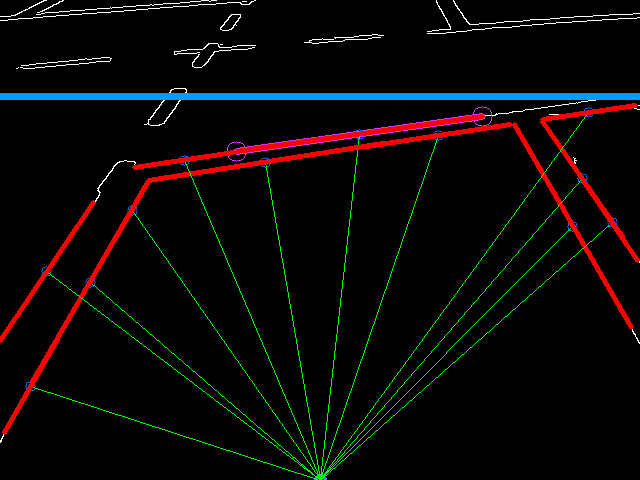
\includegraphics[width=0.8\textwidth]{figures/houghref.png}
    \end{figure}
        
    \vspace{0.5cm}
    
    \newpage
    
\begin{longtable}{ | p{0.08\textwidth } | p{0.17\textwidth } |  p{0.2\textwidth } |  p{0.22\textwidth } | p{0.22\textwidth } | p{0.22\textwidth } |  p{0.1\textwidth } |}  \hline

    % Row 1
    \rowcolor{subsectionC}\textbf{Test ID} 
    & \multicolumn{1}{c|}{\textbf{Requirement} }
    & \multicolumn{1}{c|}{\textbf{Description} }
    & \multicolumn{1}{c|}{\textbf{Input} }
    & \textbf{Expected Behaviour} 
    & \multicolumn{1}{c|}{\textbf{Actual Behaviour} }
    & \textbf{Pass/Fail} \\  
    
    % Row 2
    \multicolumn{1}{|c|}{VC3.1} 
    & \multicolumn{1}{c|}{V2}
    & At any point of the track, the lanes must be detected and extracted from the image.
    & Car on straight track segment
    & A straight line detected on each side of the car
    & Figure ~\ref{fig:Fig2}
    & \multicolumn{1}{c|}{Pass}\\  \hline
    
    
    \rowcolor{tableCell}\multicolumn{1}{|c|}{VC3.2} 
    & \multicolumn{1}{c|}{V2}
    & \multicolumn{1}{c|}{``''}
    & Car on left turn segment
    & A small left turning curve on the left side of the screen. A large left turning curve on the right of the screen 
    & Figure ~\ref{fig:Fig3}
    & \multicolumn{1}{c|}{Pass}\\ \hline
    
    
    \multicolumn{1}{|c|}{VC3.3} 
    & \multicolumn{1}{c|}{V2}
    & \multicolumn{1}{c|}{``''}
    & Car on right turn segment
    & A small right turning curve on the right side of the screen. A large right turning curve on the left of the screen 
    & Figure ~\ref{fig:Fig4}
    & \multicolumn{1}{c|}{Pass}\\ \hline
     
     
    \rowcolor{tableCell}\multicolumn{1}{|c|}{VC3.4} 
    &\multicolumn{1}{c|}{ V2, V3}
    & \multicolumn{1}{c|}{``''}
    & Car approaching intersection
    & Two vertical lines, one  on each side of the car, terminating at a horizontal line 
    & Figure ~\ref{fig:Fig5}
    & \multicolumn{1}{c|}{Pass}\\ \hline
    
    
    \multicolumn{1}{|c|}{VC3.5} 
    & \multicolumn{1}{c|}{V2, V5}
    & \multicolumn{1}{c|}{``''}
    & Car navigating through intersection
    & Small vertical line segments on each side of the car
    & Figure ~\ref{fig:Fig6}
    & \multicolumn{1}{c|}{Fail}\\ \hline
    
    
   \rowcolor{tableCell} \multicolumn{1}{|c|}{VC3.6} 
    & \multicolumn{1}{c|}{V6}
    & Any obstacles in the path of the vehicle must be detected
    & Obstacle ahead of car on a straight segment
    & Contours of obstacle detected
    & N/A
    & \multicolumn{1}{c|}{N/A}\\ \hline
    
    
    \multicolumn{1}{|c|}{VC3.7} 
    & \multicolumn{1}{c|}{V6}
    & \multicolumn{1}{c|}{``''}
    & Obstacle ahead of car on a turning segment
    & Contours of obstacle detected
    & N/A
    & \multicolumn{1}{c|}{N/A}\\ \hline
    
    
   \rowcolor{tableCell} \multicolumn{1}{|c|}{VC3.8} 
    & \multicolumn{1}{c|}{V5, V6}
    & \multicolumn{1}{c|}{``''}
    & Obstacle ahead of car at the intersection
    & Contours of obstacle detected
    & N/A
    & \multicolumn{1}{c|}{N/A}\\ \hline 
    
    
    \multicolumn{1}{|c|}{VC3.9} 
    & \multicolumn{1}{c|}{V5, V6}
    & \multicolumn{1}{c|}{``''}
    & Obstacle ahead of car at the intersection
    & Contours of obstacle detected
    & N/A
    & \multicolumn{1}{c|}{N/A}\\ \hline
    
    \end{longtable}
    \newpage
    
  \begin{longtable}{ | p{0.08\textwidth } | p{0.17\textwidth } |  p{0.2\textwidth } |  p{0.22\textwidth } | p{0.25\textwidth } | p{0.22\textwidth } |  p{0.1\textwidth } |}  \hline

    % Row 1
    \rowcolor{subsectionC}\textbf{Test ID} 
    & \multicolumn{1}{c|}{\textbf{Requirement} }
    & \multicolumn{1}{c|}{\textbf{Description} }
    & \multicolumn{1}{c|}{\textbf{Input} }
    & \textbf{Expected Behaviour} 
    & \multicolumn{1}{c|}{\textbf{Actual Behaviour} }
    & \textbf{Pass/Fail} \\  

    
    \multicolumn{1}{|c|}{VC3.10} 
    & \multicolumn{1}{c|}{V2}
    & The geometry of the captured image must be valid in order to correctly deduce logic and navigate the vehicle
    & Car on straight track segment and centered on its lane
    & leftAngle $\approx$ rightAngle \newline
      leftLength $\approx$ rightLength \newline
      intersectionDetect = 0 \newline
      obstacleDetect = 0
    & leftAngle = 42.81 \newline
      rightAngle = 40.96 \newline
      leftLength = 358.31 \newline
      rightLength = 361.45 \newline
      intersectionDetect = 0 \newline
      obstacleDetect = 0 
    & \multicolumn{1}{c|}{Pass}\\ \hline
    
    
    \rowcolor{tableCell}\multicolumn{1}{|c|}{VC3.11} 
    & \multicolumn{1}{c|}{V2}
    & \multicolumn{1}{c|}{``''}
    & Car on straight track segment and off-centered to the left
    & leftAngle $\approx$ rightAngle \newline
      leftLength $\ll$ rightLength \newline
      intersectionDetect = 0 \newline
      obstacleDetect = 0
    & leftAngle = 47.84 \newline
      rightAngle = 43.62 \newline
      leftLength = 464.34 \newline
      rightLength = 279.36 \newline
      intersectionDetect = 0 \newline
      obstacleDetect = 0 
    & \multicolumn{1}{c|}{Pass}\\ \hline
    
    
    \multicolumn{1}{|c|}{VC3.12} 
    & \multicolumn{1}{c|}{V2}
    & \multicolumn{1}{c|}{``''}
    & Car on a left turn and centered on its lane
    & leftAngle $\ll$ rightAngle \newline
      leftLength $\ll$ rightLength \newline
      intersectionDetect = 0 \newline
      obstacleDetect = 0
    & leftAngle = 24.50 \newline
      rightAngle = 51.34 \newline
      leftLength = 335.14 \newline
      rightLength = 408.33 \newline
      intersectionDetect = 0 \newline
      obstacleDetect = 0 
    & \multicolumn{1}{c|}{Pass}\\ \hline
    
    
    \rowcolor{tableCell}\multicolumn{1}{|c|}{VC3.13} 
    & \multicolumn{1}{c|}{V2}
    & \multicolumn{1}{c|}{``''}
    & Car on a right turn and centered on its lane
    & leftAngle $\gg$ rightAngle \newline
      leftLength $\gg$ rightLength \newline
      intersectionDetect = 0 \newline
      obstacleDetect = 0
    & leftAngle = 64.12 \newline
      rightAngle = 10.43 \newline
      leftLength = 377.55 \newline
      rightLength = 291.06 \newline
      intersectionDetect = 0 \newline
      obstacleDetect = 0 
    & \multicolumn{1}{c|}{Pass}\\ \hline
    
    
    
    \multicolumn{1}{|c|}{VC3.14} 
    & \multicolumn{1}{c|}{V2, V3, V4}
    & \multicolumn{1}{c|}{``''}
    & Car approaching intersection
    & leftAngle $\approx$ rightAngle \newline
      leftLength $\approx$ rightLength \newline
      intersectionDetect = 1 \newline
      obstacleDetect = 0
    & leftAngle = 67.44 \newline
      rightAngle = 61.23 \newline
      leftLength = 332.12 \newline
      rightLength = 396.56 \newline
      intersectionDetect = 1 \newline
      obstacleDetect = 0 
    & \multicolumn{1}{c|}{Pass}\\ \hline
    
    
    
    \rowcolor{tableCell}\multicolumn{1}{|c|}{VC3.15} 
    & \multicolumn{1}{c|}{V2, V6}
    & \multicolumn{1}{c|}{``''}
    & Car approaching an obstacle on a straight line segment
    & leftAngle $\approx$ rightAngle \newline
      leftLength $\approx$ rightLength \newline
      intersectionDetect = 0 \newline
      obstacleDetect = 1
    & N/A
    & \multicolumn{1}{c|}{N/A}\\ \hline
     
    \end{longtable}
    
        
% V2: The vehicle must be able to detect lanes and follow them
% V3: The vehicle must be able to detect intersections
% V4: The vehicle must be able to stop at intersections
% V5: The vehicle must be able to navigate through intersections
% V6: The vehicle must be able to avoid obstacles
\newpage






% Intersection Module Stuff
\subsubsection{Intersection Controller Software Verification} 

\textbf{5.2.2.1 Communication - Receive}\\ 
Car:
\begin{itemize}[topsep=0pt]
    \itemsep -3pt
    \item Abstract data type that contains all pertinent car request information
    \item This object is created for each new vehicle request
    \item Fields:  car\_ID, destination\_Port, destination\_bluetooth\_address, direction\_from, direction\_to,\\ proceed\_status and proceed\_message and time\_stamp
\end{itemize}

Arrival Queue:
\begin{itemize}[topsep=0pt]
    \itemsep -3pt
    \item Queue that preserves the order of the intersection requests in the form of Car objects \\
\end{itemize}

    Note: This module is currently not complete.\\
    
 %\begin{longtable}{ |p{0.08\textwidth }  |   p{0.22\textwidth } | p{0.22\textwidth } | p{0.22\textwidth } |  p{0.122\textwidth } |}  \hline
  \begin{longtable}{ | p{0.08\textwidth } | p{0.17\textwidth } |  p{0.2\textwidth } |  p{0.22\textwidth } | p{0.22\textwidth } | p{0.22\textwidth } |  p{0.1\textwidth } |}  \hline

    % Row 1
    \rowcolor{subsectionC}\textbf{Test ID}
    & \multicolumn{1}{c|}{\textbf{Requirement} }
    &\multicolumn{1}{c|}{\textbf{Description} }
    & \multicolumn{1}{c|}{\textbf{Input} }
    & \textbf{Expected Behaviour} 
    & \multicolumn{1}{c|}{\textbf{Actual Behaviour} }
    & \multicolumn{1}{c|}{\textbf{Pass/Fail}} \\  \hline
    
    % Row 2
    \multicolumn{1}{|c|}{IC1.1} 
    & \multicolumn{1}{c|}{IC1, IC5}
    & Intersection request has been sent to the intersection controller from a single vehicle
    & Single vehicle intersection request 
    & Car object containing the request information pushed into the arrival queue
    & N/A
    & \multicolumn{1}{c|}{N/A}\\ \hline
    % Row 2 
    \rowcolor{tableCell}\multicolumn{1}{|c|}{IC1.2} 
    & \multicolumn{1}{c|}{IC1, IC5}
    & Two vehicles arrive at the intersection at the same time and request to proceed through the intersection. 
    & More than one vehicle intersection request 
    & Car objects containing the request information pushed to the arrival queue in the order that they were received 
    & N/A
    & \multicolumn{1}{c|}{N/A}\\ \hline
    
    % Row 3 (without color)
    \multicolumn{1}{|c|}{IC1.3} 
    & \multicolumn{1}{c|}{IC1, IC5}
    & Vehicle intersection requests that are transmitted incompletely should be dropped by it intersection controller
    &  Vehicle intersection request that is terminated prior to receive completion
    & Timeout/ disconnected receive error is caught and system becomes available for subsequent requests
    & N/A
    & \multicolumn{1}{c|}{N/A}\\ \hline 
    
    
    
  
  
    
     % Row 4
    \rowcolor{tableCell}\multicolumn{1}{|c|}{IC1.4} 
    & \multicolumn{1}{c|}{IC1, IC5}
    & The system should be able to handle large request volumes without losing requests. 
    & Many vehicle requests
    &  Car objects containing the request information pushed to the arrival queue in the order that they were received 
    & N/A
    & \multicolumn{1}{c|}{N/A}\\ \hline
    \newpage \hline


    
    % Row 4 (without color)
    \multicolumn{1}{|c|}{IC1.5} 
    & \multicolumn{1}{c|}{IC1}
    & Messages that have invalid or corrupt message contents should be dropped
    & Invalid message \newline request
    & Invalid/corrupt message detected and dropped
    & N/A
    & \multicolumn{1}{c|}{N/A}\\ \hline
     
    \end{longtable}
    
    \textbf{5.2.2.2 Communication - Send}  \\ 
    
    Proceed Queue:
\begin{itemize}[topsep=0pt]
    \itemsep -3pt
    \item Queue of car objects that preserves the order determined by the intersection controller that vehicles should proceed through the intersection. 
    \item Proceed commands are sent to the vehicles based on the FIFO sequence of the proceed queue\\
\end{itemize}

    Note: This module is currently not complete.\\
    
    
 \begin{longtable}{ | p{0.08\textwidth } | p{0.17\textwidth } |  p{0.2\textwidth } |  p{0.22\textwidth } | p{0.22\textwidth } | p{0.22\textwidth } |  p{0.1\textwidth } |}  \hline

    % Row 1
    \rowcolor{subsectionC}\textbf{Test ID}
    & \multicolumn{1}{c|}{\textbf{Requirement} }
    &\multicolumn{1}{c|}{\textbf{Description} }
    & \multicolumn{1}{c|}{\textbf{Input} }
    & \textbf{Expected Behaviour} 
    & \multicolumn{1}{c|}{\textbf{Actual Behaviour} }
    & \multicolumn{1}{c|}{\textbf{Pass/Fail}} \\  \hline
    
    % Row 2
   
    \multicolumn{1}{|c|}{IC2.1} 
    & \multicolumn{1}{c|}{IC5}
    & Vehicle proceed request has been determined safe and must be communicated to the vehicle
    & Car object in the proceed queue
    & Remove vehicle from proceed queue and send proceed message to vehicle 
    & N/A
    & \multicolumn{1}{c|}{N/A}\\ \hline
    
    % Row 2 
  
    \rowcolor{tableCell}\multicolumn{1}{|c|}{IC2.2} 
    & \multicolumn{1}{c|}{V1, IC4, IC5}
    & Multiple vehicle proceed requests have been determined safe and must be communicated to the vehicle
    & More than one car object in the proceed queue
    & Remove vehicles from departure queue and send proceed message to vehicles in FIFO order.  
    & N/A
    & \multicolumn{1}{c|}{N/A}\\ \hline
    
    
    % Row 3
    \multicolumn{1}{|c|}{IC2.3} 
    & \multicolumn{1}{c|}{IC5}
    & The system should be able to handle large send volumes without dropping proceed commands
    & Many vehiles in the proceed queue
    & ``''
    & N/A
    & \multicolumn{1}{c|}{N/A}\\ \hline
    
    
   
    % Row 4 
    \rowcolor{tableCell}\multicolumn{1}{|c|}{IC2.4} 
    & \multicolumn{1}{c|}{IC5}
    & System should make further attempts to transmit messages to an unresponsive connection  up to a max limit 
    & Car object in the proceed queue
    & Inactive connection error should be caught. The system should then attempt to send the message again (up to the maximum attempt limit)
    & N/A
    & \multicolumn{1}{c|}{N/A}\\  \hline
    
    \pagebreak \hline
   
    
    % Row 5 (without color)
    \multicolumn{1}{|c|}{IC2.5} 
    & \multicolumn{1}{c|}{IC5}
    & ``''
    & ``'' 
    &  Timeout/ disconnected send error should be caught.  The system should then attempt to send the message again (up to the maximum attempt limit)
    & N/A
    & \multicolumn{1}{c|}{N/A}\\ \hline
    
    \end{longtable}
    
     \textbf{5.2.2.3 Communication - Message Extraction} 
     
     Note: This module is currently not complete.\\
     
 \begin{longtable}{ | p{0.08\textwidth } | p{0.17\textwidth } |  p{0.2\textwidth } |  p{0.22\textwidth } | p{0.22\textwidth } | p{0.22\textwidth } |  p{0.1\textwidth } |}  \hline

    % Row 1
    \rowcolor{subsectionC}\textbf{Test ID}
    & \multicolumn{1}{c|}{\textbf{Requirement} }
    &\multicolumn{1}{c|}{\textbf{Description} }
    & \multicolumn{1}{c|}{\textbf{Input} }
    & \multicolumn{1}{c|}{\textbf{Expected Values} }
    & \multicolumn{1}{c|}{\textbf{Actual Values} }
    & \multicolumn{1}{c|}{\textbf{Pass/Fail}} \\  \hline
    
    % Row 2
       \multicolumn{1}{|c|}{IC3.1} 
    & \multicolumn{1}{c|}{IC5}
    &Vehicle message contents are separated by an agreed upon separator
    % input is client message with destination port number, arriving from, going to
    % client address doesn't need to be transmitted in the request as this can be retrieved when
    % the connection is made
    & 2\_N\_S\_1\_timestamp
    % expected output is a car object with destination bluetooth id, port number, arriving from, and going to
    & Car(2, bluetooth Address, 1, 'N', 'S', `', `', 'timestamp') 
    &  N/A
    & \multicolumn{1}{c|}{N/A}\\\hline
    
    
    % Row 3
    \rowcolor{tableCell}\multicolumn{1}{|c|}{IC3.2} 
    & \multicolumn{1}{c|}{IC5} 
    &The intersection communication module should drop incomplete or corrupt message contents
    & 2\_N\_N\_1\_timestamp
    & Incorrect Message contents error caught
    &  N/A
    & \multicolumn{1}{c|}{N/A}\\\hline
    
    % Row 4
    \multicolumn{1}{|c|}{IC3.3} 
    & \multicolumn{1}{c|}{IC5} 
    & ``''
    & 2\_N\_N\_1\_
    & Incorrect Message contents error caught
    &  N/A
    & \multicolumn{1}{c|}{N/A}\\ \hline
    
    \end{longtable}
    
    
    \textbf{5.2.2.4 ImageProcessing} \vspace{2mm}\\
    Note: This module is not yet completed. 
    
    
  \begin{longtable}{ | p{0.08\textwidth } | p{0.17\textwidth } |  p{0.2\textwidth } |  p{0.22\textwidth } | p{0.22\textwidth } | p{0.22\textwidth } |  p{0.1\textwidth } |}  \hline

    % Row 1
    \rowcolor{subsectionC}\textbf{Test ID}
    & \multicolumn{1}{c|}{\textbf{Requirement} }
    &\multicolumn{1}{c|}{\textbf{Description} }
    & \multicolumn{1}{c|}{\textbf{Input} }
    & \textbf{Expected Behaviour} 
    & \multicolumn{1}{c|}{\textbf{Actual Behaviour} }
    & \multicolumn{1}{c|}{\textbf{Pass/Fail}} \\  \hline
    
    % Row 2
    \multicolumn{1}{|c|}{IC4.1} 
    &\multicolumn{1}{c|}{IC5}  
    & The IC must be able to detect when there are the intersection is occupied
    & Video frame of the intersection with no cars on the track
    & The module determines that there are no cars in the intersection  
    & N/A
    &\multicolumn{1}{c|}{N/A}\\ \hline
    
    % Row 2 (with color)
    \rowcolor{tableCell}\multicolumn{1}{|c|}{IC4.2} 
    &\multicolumn{1}{c|}{IC3, IC5} 
    & \multicolumn{1}{c|}{" "} 
    & Video frame of intersection with a car in the intersection
    & Module determines the intersection is occupied
    & N/A
    & \multicolumn{1}{c|}{N/A}\\ \hline
    
    \newpage\hline
    
    % Row 3 (without color)
    \multicolumn{1}{|c|}{IC4.3} 
    &\multicolumn{1}{c|}{IC3, IC5}
    & \multicolumn{1}{c|}{" "} 
    & Video frame of car leaving the intersection
    & The module changes the intersection from occupied to unoccupied
    & N/A
    & \multicolumn{1}{c|}{N/A}\\ \hline
    
     % Row 4
    \rowcolor{tableCell}\multicolumn{1}{|c|}{IC4.4} 
        &\multicolumn{1}{c|}{IC5}  
    &\multicolumn{1}{c|}{" "} 
    & Video frame of a stationary obstacle in the intersection
    & The module determines that the intersection is occupied indefinately
    & N/A
    & \multicolumn{1}{c|}{N/A}\\ \hline
    
    % Row 5 (without color)
    \multicolumn{1}{|c|}{IC4.5} 
    &\multicolumn{1}{c|}{IC3}
    & The intersection must determine which car has navigated through the intersection using directions
    & Video clip showing vehicle proceeding from North to South of the intersection
    & The module records the movement 
    & N/A
    & \multicolumn{1}{c|}{N/A} \\\hline
    
    % Row 6 (with color)
    \rowcolor{tableCell}\multicolumn{1}{|c|}{IC4.6} 
    &\multicolumn{1}{c|}{IC3}
    & \multicolumn{1}{c|}{" "} 
    & Video clip showing vehicle proceeding from South to North of the intersection
    & The module records the movement 
    & N/A
    & \multicolumn{1}{c|}{N/A} \\\hline
    
    % Row 5 (without color)
    \multicolumn{1}{|c|}{IC4.7} 
    &\multicolumn{1}{c|}{IC3}
     & \multicolumn{1}{c|}{" "} 
    & Video clip showing vehicle proceeding from East to West of the intersection
    & The module records the movement 
    & N/A
    & \multicolumn{1}{c|}{N/A} \\\hline
    
    % Row 6 (with color)
    \rowcolor{tableCell}\multicolumn{1}{|c|}{IC4.8} 
    &\multicolumn{1}{c|}{IC3}
    & \multicolumn{1}{c|}{" "} 
    & Video clip showing vehicle proceeding from West to East of the intersection
    & The module records the movement 
    & N/A
    & \multicolumn{1}{c|}{N/A} \\ \hline
     
    \end{longtable}


\subsubsection{Integrated Vehicle Intersection Software Verification}
\textbf{5.2.3.1 } \vspace{2mm}

 Note: The VIC system is only partially implemented, integrated system testing will take place in the future.\\

\begin{longtable}{ | p{0.08\textwidth } | p{0.17\textwidth } |  p{0.2\textwidth } |  p{0.22\textwidth } | p{0.22\textwidth } | p{0.22\textwidth } |  p{0.1\textwidth } |}  \hline

    % Row 1
    \rowcolor{subsectionC}\textbf{Test ID}
    & \multicolumn{1}{c|}{\textbf{Requirement} }
    &\multicolumn{1}{c|}{\textbf{Description} }
    & \multicolumn{1}{c|}{\textbf{Input} }
    & \textbf{Expected Behaviour} 
    & \multicolumn{1}{c|}{\textbf{Actual Behaviour} }
    & \multicolumn{1}{c|}{\textbf{Pass/Fail}} \\  \hline
    
    % Row 2
    \multicolumn{1}{|c|}{VIC.1} 
    & \multicolumn{1}{c|}{IC1, IC5}
    &Vehicles are allowed to proceed directly through the intersection, without stopping if the intersection is deemed safe and clear
    & Single vehicle, clear intersection
    & Vehicle proceeds directly through the intersection
    & N/A 
    & \multicolumn{1}{c|}{N/A}\\ \hline
    
    \newpage\hline
    
    % Row 2 (with color)
    \rowcolor{tableCell}\multicolumn{1}{|c|}{VIC.2} 
    & \multicolumn{1}{c|}{IC1, IC4, IC5}
    & Vehicles are designed to stop at the intersection until they receive a proceed command from the intersection    
    & Single vehicle, obstacle in intersection
    & Vehicle should stop at the intersection
    & N/A
    & \multicolumn{1}{c|}{N/A}\\ \hline
    
    % Row 3 (without color)
    \multicolumn{1}{|c|}{VIC.3} 
    & \multicolumn{1}{c|}{V1}
    & ``''
    
    & Single vehicle, intersection controller system not working
    &  Vehicle should stop at the intersection and wait
    & N/A
    & \multicolumn{1}{c|}{N/A}\\ \hline
    
    
        % Row 4 
        \rowcolor{tableCell}\multicolumn{1}{|c|}{VIC.4} 
    & \multicolumn{1}{c|}{V3, IC4, IC5}
    & Vehicles are allowed to proceed directly through the intersection, without stopping if the intersection is deemed safe and clear and the intended paths are parallel
    & Multiple vehicles, parallel directions, clear intersection
    & Vehicles proceed directly through the intersection
    &  N/A
    & \multicolumn{1}{c|}{N/A}\\ \hline
    
     % Row 5
    \multicolumn{1}{|c|}{VIC.5} 
    &\begin{minipage}{.17\textwidth} \vspace{1 mm} \begin{center}
    V3, V4, V5, IC4, IC5
    \end{center}\end{minipage} 
    %\multicolumn{1}{c|}{}
    & Vehicles with crossing directions must stop at the intersection, the vehicle that arrived first proceeds through the intersection first
    &  Vehicle A and Vehicle B, crossing directions, clear intersection, Vehicle A is first
    &Vehicles A proceeds directly through the intersection, Vehicle B stops at the intersection 
    & N/A 
    & \multicolumn{1}{c|}{N/A}\\ \hline
    
    % Row 6 (without color)
    \rowcolor{tableCell}\multicolumn{1}{|c|}{VIC.6} 
    & \multicolumn{1}{c|}{V1, V3, V4}
    & Vehicles are designed to stop at the intersection until they receive a proceed command from the intersection
    & Multiple vehicles, obstacle in intersection
    & Vehicles should stop at the intersection 
    & N/A 
    & \multicolumn{1}{c|}{N/A}\\  \hline
    
     % Row 7
    \multicolumn{1}{|c|}{VIC.7} 
    & \multicolumn{1}{c|}{V1}
    & ``''
    & Multiple vehicles, intersection controller not working
    &  Vehicles should stop at the intersection and wait
    & N/A 
    & \multicolumn{1}{c|}{N/A}\\ \hline
    \end{longtable}


%%%%%%%%%%%%%%%%%%%%%%%%%%%%%%%%%%%%%%%%%

% This adds the page number to the rotated page
\begin{landscape}
\end{landscape}
\endgroup

% -------------- END Landscape Page  ---------------- %

% -------------- Reset Page  ---------------- %



    
    
\newpage
\paperwidth=\pdfpageheight
\paperheight=\pdfpagewidth
\pdfpageheight=\paperheight
\pdfpagewidth=\paperwidth
\headwidth=\textwidth



 

\section{Appendix}
\subsection{Image Processing Verification Results}

 \begin{figure}[h]
\centering
\begin{subfigure}
  \centering
  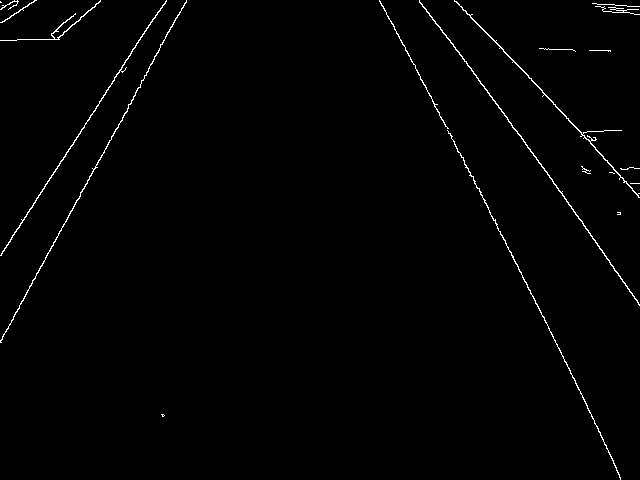
\includegraphics[width=.4\linewidth]{figures/straight_canny.png}
\end{subfigure}%
\begin{subfigure}
  \centering
  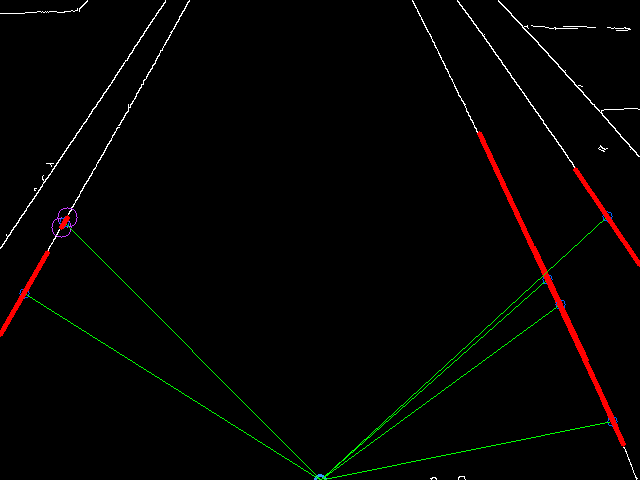
\includegraphics[width=.4\linewidth]{figures/straight_h.png}
\end{subfigure}
\caption{Straight line segment}
\label{fig:Fig2}
\end{figure}


\begin{figure}[h]
\centering
\begin{subfigure}
  \centering
  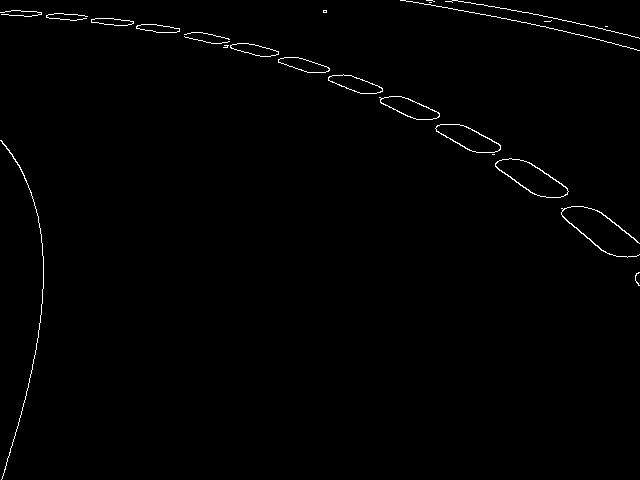
\includegraphics[width=.4\linewidth]{figures/left_c.png}
\end{subfigure}%
\begin{subfigure}
  \centering
  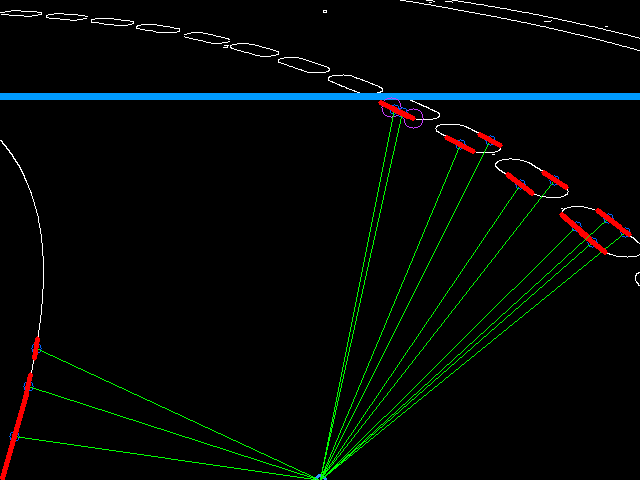
\includegraphics[width=.4\linewidth]{figures/left_h.png}
\end{subfigure}
\caption{Left turn segment}
\label{fig:Fig3}
\end{figure}

\begin{figure}
\centering
\begin{subfigure}
  \centering
  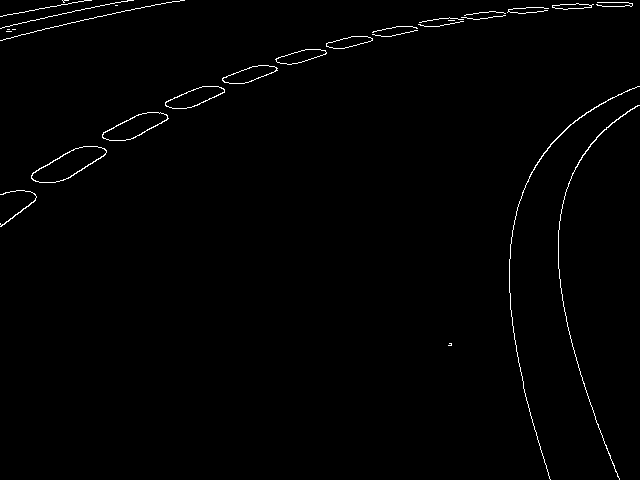
\includegraphics[width=.4\linewidth]{figures/right_c.png}
\end{subfigure}%
\begin{subfigure}
  \centering
  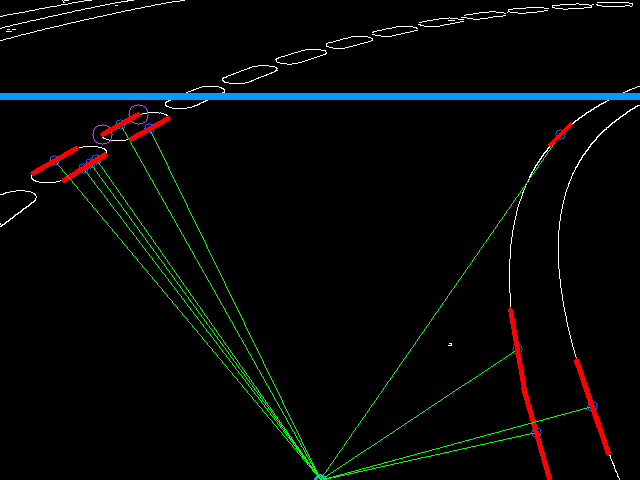
\includegraphics[width=.4\linewidth]{figures/right_h.png}
\end{subfigure}
\caption{Right turn segment}
\label{fig:Fig4}
\end{figure}

\begin{figure}
\centering
\begin{subfigure}
  \centering
  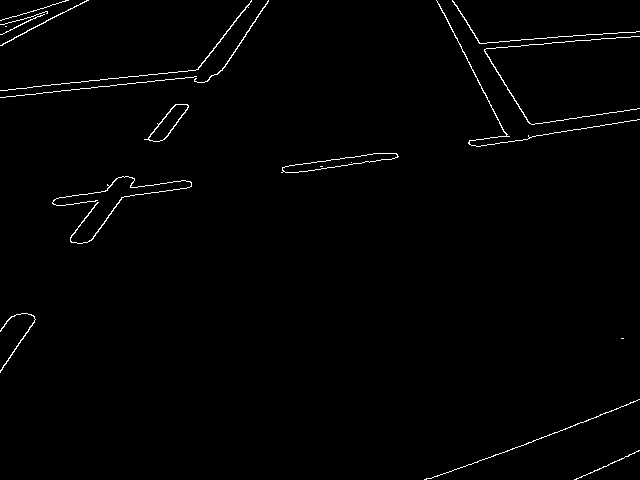
\includegraphics[width=.4\linewidth]{figures/intersection2_c.png}
\end{subfigure}%
\begin{subfigure}
  \centering
  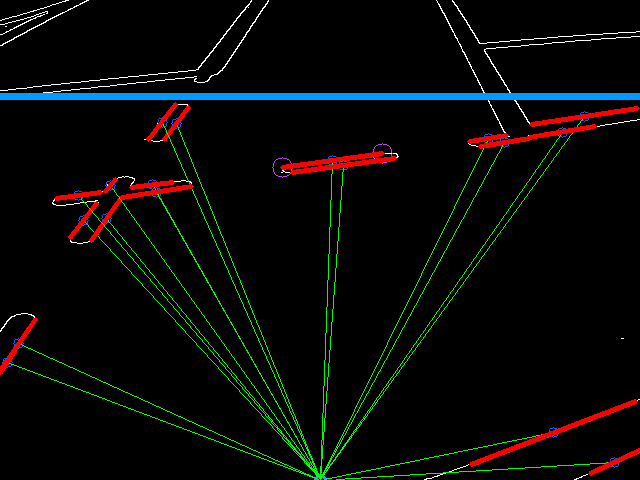
\includegraphics[width=.4\linewidth]{figures/intersection2_h.png}
\end{subfigure}
\caption{Approaching an intersection}
\label{fig:Fig5}
\end{figure}

\begin{figure}
\centering
\begin{subfigure}
  \centering
  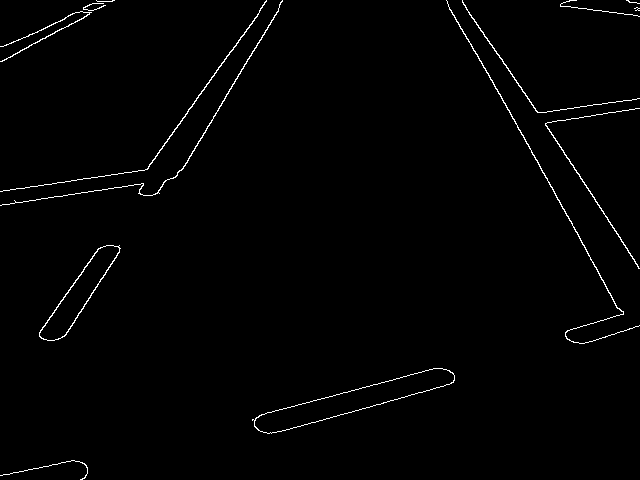
\includegraphics[width=.4\linewidth]{figures/intersection3_c.png}
\end{subfigure}%
\begin{subfigure}
  \centering
  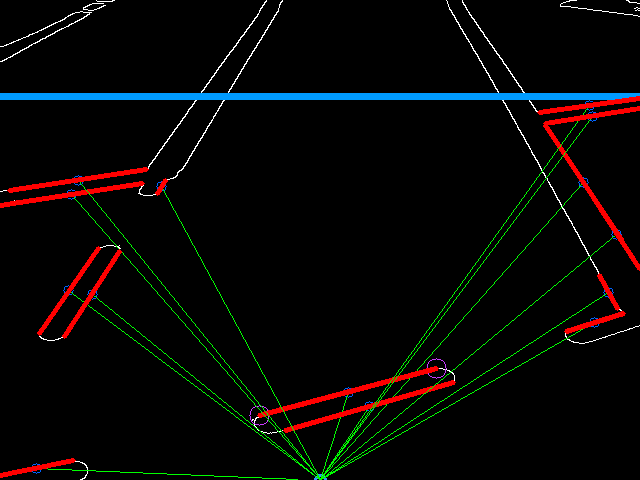
\includegraphics[width=.4\linewidth]{figures/intersection3_h.png}
\end{subfigure}
\caption{Navigating through an intersection}
\label{fig:Fig6}

\end{figure}





\end{document}


















